\documentclass[11pt]{article} 

\usepackage[utf8]{inputenc} 

%%% PAGE DIMENSIONS
\usepackage{geometry} % to change the page dimensions
\geometry{a4paper} % or letterpaper (US) or a5paper or....
\geometry{margin=1in} % for example, change the margins to 2 inches all round

\usepackage{graphicx} % support the \includegraphics command and options

%%% PACKAGES
\usepackage{booktabs} % for much better looking tables
\usepackage{array} % for better arrays (eg matrices) in maths
\usepackage{paralist} % very flexible & customisable lists (eg. enumerate/itemize, etc.)
\usepackage{verbatim} % adds environment for commenting out blocks of text & for better verbatim
%\usepackage{subfig} % make it possible to include more than one captioned figure/table in a single float
\usepackage{enumitem}
\usepackage{multicol}
\usepackage{tikz}
\usepackage{subcaption}
\usepackage{multirow}
\usepackage[brazilian]{babel}
\usepackage[siunitx]{circuitikz}
\tikzset{
  declare function={% in case of CVS which switches the arguments of atan2
    atan3(\a,\b)=ifthenelse(atan2(0,1)==90, atan2(\a,\b), atan2(\b,\a));},
  kinky cross radius/.initial=+.125cm,
  @kinky cross/.initial=+, kinky crosses/.is choice,
  kinky crosses/left/.style={@kinky cross=-},kinky crosses/right/.style={@kinky cross=+},
  kinky cross/.style args={(#1)--(#2)}{
    to path={
      let \p{@kc@}=($(\tikztotarget)-(\tikztostart)$),
          \n{@kc@}={atan3(\p{@kc@})+180} in
      -- ($(intersection of \tikztostart--{\tikztotarget} and #1--#2)!%
             \pgfkeysvalueof{/tikz/kinky cross radius}!(\tikztostart)$)
      arc [ radius     =\pgfkeysvalueof{/tikz/kinky cross radius},
            start angle=\n{@kc@},
            delta angle=\pgfkeysvalueof{/tikz/@kinky cross}180 ]
      -- (\tikztotarget)}}}

%%% HEADERS & FOOTERS
\usepackage{fancyhdr} % This should be set AFTER setting up the page geometry
\pagestyle{fancy} % options: empty , plain , fancy
\renewcommand{\headrulewidth}{0pt} % customise the layout...
\lhead{}\chead{Universidade Federal Fluminense\\Departamento de Engenharia Elétrica\\TEE00129 - Laboratório de Eletrônica Básica}\rhead{}
\lfoot{}\cfoot{\thepage}\rfoot{}

%%% SECTION TITLE APPEARANCE
%\usepackage{sectsty}
%\allsectionsfont{\sffamily\mdseries\upshape} % (See the fntguide.pdf for font help)

%%% ToC (table of contents) APPEARANCE
\usepackage[nottoc,notlof,notlot]{tocbibind} % Put the bibliography in the ToC
\usepackage[titles,subfigure]{tocloft} % Alter the style of the Table of Contents
\renewcommand{\cftsecfont}{\rmfamily\mdseries\upshape}
\renewcommand{\cftsecpagefont}{\rmfamily\mdseries\upshape} % No bold!

%%% END Article customizations

\title{Aula 5: Amplificador Emissor Comum}
\author{Prof. Derick Furquim Pereira}
\date{} % Activate to display a given date or no date (if empty),
         % otherwise the current date is printed 

\begin{document}
\maketitle
\thispagestyle{fancy}

\section*{Parte teórica}

\subsection*{Questionário}

\begin{enumerate}

\item (4,0) Dado o circuito do amplificador de emissor comum na Figura \ref{circ1} abaixo, determine o seu ganho de tensão ($V_{out}/V_{in}$). Dados: $V_{in}=5\sin(2\pi1000t)$ mV.
\begin{figure}[!h]
	\centering
	\begin{circuitikz}[american voltages,scale=.6, transform shape]
	\draw
	% Drawing a npn transistor
	(0,0) node[npn](npn1){}
	% Making connections from transistor using relative coordinates
	(npn1.B) -- ++(-1,0) node(base){}
	(npn1.B) -- ++(-1,0) to [R,l=10<\kilo\ohm>,*-] 
				++(0,3) node(con1){}
	(0,3) node(con2){}
	(npn1.B) -- ++(-1,0) to [R,l_=2.2<\kilo\ohm>,*-] ++(0,-3) node(gnd1){}
	(npn1.B) -- ++(-1,0) to [C,l=1<\micro\farad>] 
				++(-2,0) to [R,l=15<\kilo\ohm>] 
				++(-3,0) to[sV,l_=$V_{in}$] 
				++(0,-3) to[short,-*] 
				++(5,0)
	(npn1.E)	to [R,l=820<\ohm>,*-] (0,-3)
	(npn1.E)	to [short] ++(2,0)
				to [C,l=47<\micro\farad>] (2,-3) 
				to [short] (0,-3)
	(con2)	to [R,l=3.9<\kilo\ohm>,-*] (npn1.C)
			to [C,-*,l_=1<\micro\farad>] ++(2,0) node[right]{$V_{out}$}
	% Drawing shorts and ground connection
	(0,3)	to[short,*-o] (0,4) node[right]{$V_{CC}=+12 V$} % Power supply
	(0,-3) node[ground]{}% Define this node as ground
	(gnd1) ++(0,0) to[short,-*] ++(1.85,0)
	(con1)	to[short] ++(1.85,0)
	(base)	to[short] ++(1,0)
%	(npn1.C) node[anchor=west]{C}
%	(base) node[anchor=east]{B}
%	(npn1.E) node[anchor=west]{E}
	;
	\end{circuitikz}
	\caption{Circuito do amplificador emissor comum.}
	\label{circ1}
\end{figure}

\end{enumerate}

\section*{Verificação do ganho de tensão do amplificador}

\subsection*{Procedimento}

Coloque as chaves S1, S2 e S5 do \textit{DIP Switch} na posição fechada (ON) e mantenha as demais chaves na posição aberta. Nesta condição, tem-se o circuito equivalente mostrado na Figura \ref{circ2}.

\begin{figure}[!htb]
\centering
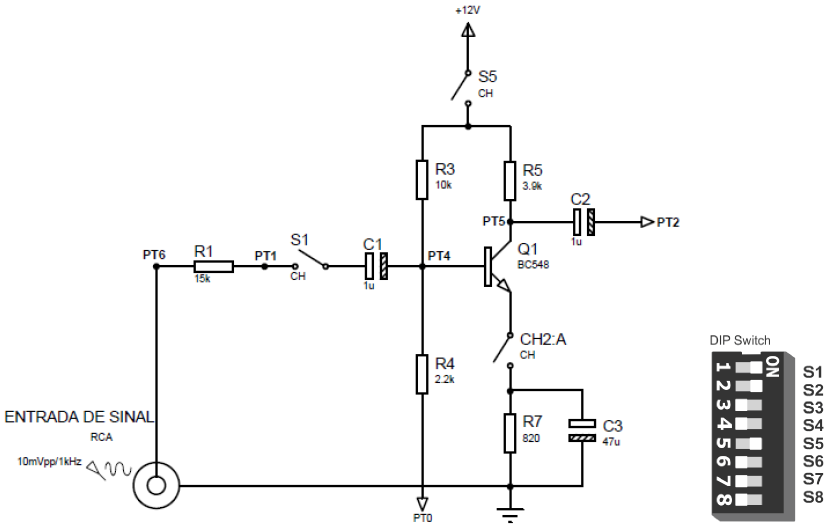
\includegraphics[width=.65\textwidth]{AmplificadorEmissorComum.png}
\caption{Circuito para observar as características de transferência.}
\label{circ2}
\end{figure}

Selecione o gerador de funções do módulo em frequência baixa, sinal senoidal e ligue o módulo.

\subsection*{Questionário}

\begin{enumerate}
\setcounter{enumi}{1}

\item (1,5) Com o auxílo de um osciloscópio, ajuste o sinal de entrada (PT6) para amplitude em torno de 10 mV pico a pico e frequência de 1 kHz aproximadamente. Esboce a forma de onda observada e meça os valores de pico a pico, eficaz, médio, o período e a frequência.

\begin{figure}[!h]
	\centering
	\begin{tikzpicture}
		\draw[step=.5cm,gray,very thin] (0,0) grid (5,4);	
	\end{tikzpicture}
\end{figure}

\begin{table}[!h]
\centering
%\caption{Tensão de saída do retificador de onda completa com derivação central.}
\begin{tabular}{|c|c|c|c|c|}
\hline
Valor & Acoplamento CC & Acoplamento CA & Período & Frequência\\\hline
Pico-pico & & & & \\\cline{1-3}
Eficaz & & & & \\\cline{1-3}
Médio & & & & \\\hline
\end{tabular}
\end{table}
	\item (1,5) Com o auxílio de um osciloscópio, meça o valor médio da tensão na base do transistor Q1 (PT4) da Figura \ref{circ2} e compare com o valor teórico calculado na questão 1 feita na parte teórica.
	\item (1,5) Com o auxílio de um osciloscópio, observe o sinal de saída do amplificador emissor comum da Figura \ref{circ2} e responda as questões abaixo.
	\begin{enumerate}
		\item Meça e anote o valor de pico a pico da tensão de saída no terminal do coletor (PT5).
		\item Calcule o ganho de tensão do amplificador.
	\end{enumerate}
	\item (1,5) Aumente gradualmente a amplitude do sinal de entrada e, ao mesmo tempo, observe o sinal de saída com o auxílio de um osciloscópio. Meça o valor de pico a pico da tensão de entrada (PT1), para o qual a saída (PT2) começa a saturar.
\end{enumerate}

\end{document}
